\subsection{Progettazione di dettaglio e codifica}
Questa fase comincia in seguito al termine della precedente e si conclude con la \textit{Revisione di Qualifica}, ovvero dal 08-03-2021 al 02-04-2021. Durante questa fase verranno implementate buona parte delle componenti della \glo{web app} e verranno anche aggiunte funzionalità alle componenti già sviluppate in precedenza.
Di seguito è riportato ogni incremento in dettaglio.

\subsubsection{Incremento III} 

\paragraph{Obiettivi}
\begin{itemize}
\item Implementazione di un componente per applicare una riduzione dimensionale ai dati  \textbf{[UC3]};
\item Aggiunta di alcuni controlli per la configurazione dei parametri relativi ai diversi algoritmi di riduzione dimensionale disponibili \textbf{[UC4]}.
\item Consolidamento del design pattern architetturale.
\end{itemize}

\paragraph{Periodi e attività} \mbox{}\\\mbox{}\\
Questo incremento si compone di un unico periodo, dal 08-03-2021 al 13-03-2021, con milestone fissata per l'ultimo giorno. Comprende attività di:
\begin{itemize}
\item \textbf{Stesura:} eventuali correzioni e integrazioni ai documenti;
\item \textbf{Verifica documenti};
\item \textbf{Progettazione:} progettazione del componente per la riduzione dimensionale;
\item \textbf{Codifica:} codifica del componente per la riduzione dimensionale con relativa parametrizzazione;
\item \textbf{Verifica software:} verifica sulle funzionalità software aggiunte.
\end{itemize}

\subsubsection{Incremento IV}

\paragraph{Obiettivi}
\begin{itemize}
\item Implementazione della visualizzazione \glo{Adjacency Matrix} \textbf{[UC5.2]};
\item Aggiunta di alcuni controlli per la configurazione dei parametri relativi alla visualizzazione precedentemente implementata \textbf{[UC5.3]}.
\end{itemize}

\paragraph{Periodi e attività} \mbox{}\\\mbox{}\\
Questo incremento si compone di un unico periodo, dal 13-03-2021 al 17-03-2021, con milestone fissata per l'ultimo giorno. Comprende attività di:
\begin{itemize}
\item \textbf{Stesura:} eventuali correzioni e integrazioni ai documenti;
\item \textbf{Verifica documenti};
\item \textbf{Progettazione:} progettazione del componente per la visualizzazione \glo{Adjacency Matrix};
\item \textbf{Codifica:} codifica del componente per la visualizzazione con relativa parametrizzazione;
\item \textbf{Verifica software:} verifica sulle funzionalità software aggiunte.
\end{itemize}


\subsubsection{Incremento V}

\paragraph{Obiettivi}
\begin{itemize}
\item Implementazione della visualizzazione \glo{Force Field} \textbf{[UC5.3]};
\item Aggiunta di alcuni controlli per la configurazione dei parametri relativi alla visualizzazione precedentemente implementata \textbf{[UC6.3]}.
\end{itemize}

\paragraph{Periodi e attività} \mbox{}\\\mbox{}\\
Questo incremento si compone di un unico periodo, dal 17-03-2021 al 21-03-2021, con milestone fissata per l'ultimo giorno. Comprende attività di:
\begin{itemize}
\item \textbf{Stesura:} incremento della documentazione da allegare al prodotto e inizio del manuale utente e del manuale manutentore;
\item \textbf{Verifica documenti};
\item \textbf{Progettazione:} progettazione del componente per la visualizzazione \glo{Force Field};
\item \textbf{Codifica:} codifica del componente per la visualizzazione con relativa parametrizzazione;
\item \textbf{Verifica software:} verifica sulle funzionalità software aggiunte.
\end{itemize}

\subsubsection{Incremento VI}

\paragraph{Obiettivi}
\begin{itemize}
\item Implementazione della visualizzazione \glo{Proiezione Lineare Multi Asse} e \glo{HeatMap} \textbf{[UC5.4, UC5.5]};
\item Aggiunta di alcuni controlli per la configurazione dei parametri relativi alla visualizzazione precedentemente implementata \textbf{[UC6.4, UC6.5]}.
\end{itemize}

\paragraph{Periodi e attività} \mbox{}\\\mbox{}\\
Questo incremento si compone di un unico periodo, dal 21-03-2021 al 26-03-2021, con milestone fissata per l'ultimo giorno. Comprende attività di:
\begin{itemize}
\item \textbf{Stesura:} incremento della documentazione da allegare al prodotto ;
\item \textbf{Verifica documenti};
\item \textbf{Progettazione:} progettazione dei componenti per la visualizzazione \glo{PLMA} e \glo{HeatMap};
\item \textbf{Codifica:} codifica dei componenti per le visualizzazioni con relative parametrizzazioni;
\item \textbf{Verifica software:} verifica sulle funzionalità software aggiunte.
\end{itemize}

\newpage
\subsubsection{Incremento VII}

\paragraph{Obiettivi}
\begin{itemize}
\item Implementazione di un database;
\item Sviluppo di un componente per la scelta e il caricamento di un \glo{dataset} contenuto nel \glo{database} \textbf{[UC1.1.2]}.
\end{itemize}

\paragraph{Periodi e attività} \mbox{}\\\mbox{}\\
Questo incremento si compone di un unico periodo, dal 26-03-2021 al 02-04-2021, con milestone fissata per l'ultimo giorno. Comprende attività di:
\begin{itemize}
\item \textbf{Stesura:} incremento e conclusione della documentazione da allegare al prodotto;
\item \textbf{Verifica documenti};
\item \textbf{Progettazione:} progettazione del \glo{database} e del componente per la scelta e il caricamento del \glo{dataset};
\item \textbf{Creazione struttura database:} stesura della struttura del \glo{database};
\item \textbf{Codifica:} codifica del componente per la scelta e il caricamento del \glo{dataset};
\item \textbf{Verifica software:} verifica sulle funzionalità software aggiunte.
\end{itemize}

\begin{landscape}

\begin{figure}[h]
 	\centering
	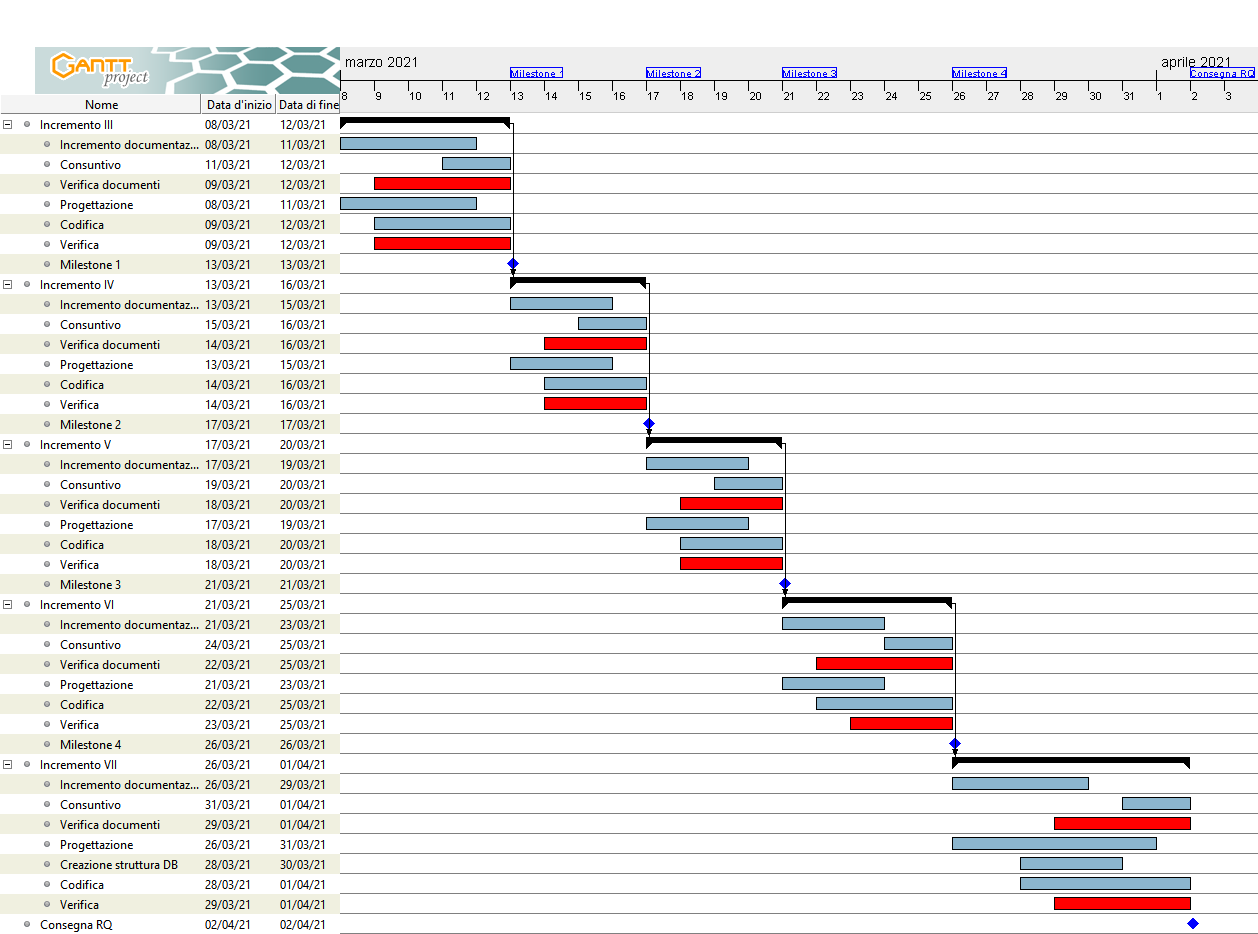
\includegraphics[width=\linewidth]{Images/GanttPianificazioneProgettazioneDettaglioCodifica.png}
	\caption{Diagramma di Gantt dell'attività di progettazione di dettaglio e codifica}
\end{figure}

\end{landscape}